\documentclass{article}
\usepackage[utf8]{inputenc}
\usepackage{graphicx}
\usepackage{booktabs}
\usepackage{float}
\graphicspath{ {./metrics/fold_0/} }
\graphicspath{ {./metrics/fold_1/} }
\graphicspath{ {./metrics/fold_2/} }
\title{Results: mirim-mech-[bert]-lr-[0.00005|0.00001|0.000001]}
\author{Nadia Sheikh}
\date{2022-07-25}
\begin{document}
\maketitle
\section{Configurations}
\subsection{Run Configuration}
\begin{tabular}{ll}
\toprule
{} &                                                  0 \\
\midrule
experiment\_identifier &                                              mirim \\
run\_identifier        &    mirim-mech-[bert]-lr-[0.00005|0.00001|0.000001] \\
config\_file\_path      &  /home/nadia/Documents/CLaC-Lab/ctre/cnc-task-3... \\
\bottomrule
\end{tabular}

\subsection{Data Configuration}
\begin{tabular}{ll}
\toprule
{} &                                                  0 \\
\midrule
data\_utility\_cls        &                                      cnc\_utilities \\
dataset\_cls             &                                   CNCTask3aDataset \\
nos\_of\_folds            &                                                  3 \\
trn\_data\_path           &    /cnc-task-3/script-development/data/CSV-Output/ \\
tst\_data\_path           &  /home/nadia/Documents/CLaC-Lab/ctre/cnc-task-3... \\
base\_output\_folder\_path &             /cnc-task-3/script-development/output/ \\
config\_file\_path        &  /home/nadia/Documents/CLaC-Lab/ctre/cnc-task-3... \\
\bottomrule
\end{tabular}

\subsection{Preprocessing Configuration}
\begin{tabular}{ll}
\toprule
{} &                                                  0 \\
\midrule
collate\_fn\_name   &                                       LLMCollateFn \\
llm\_name          &                                  bert-base-uncased \\
connl\_folder\_path &  /home/nadia/Documents/CLaC-Lab/ctre/cnc-task-3... \\
max\_nos\_tokens    &                                                 84 \\
token\_sep         &                                               True \\
config\_file\_path  &  /home/nadia/Documents/CLaC-Lab/ctre/cnc-task-3... \\
\bottomrule
\end{tabular}

\section{Hyperparameters}
\subsection{hparam\_config\_id\_0}
\begin{tabular}{ll}
\toprule
{} &                   0 \\
\midrule
loss\_function                    &  cross-entropy-loss \\
learning\_rate                    &             0.00001 \\
batch\_size                       &                   1 \\
optimizer                        &                adam \\
llm                              &   bert-base-uncased \\
llm\_hidden\_dropout\_prob          &                 0.1 \\
llm\_attention\_probs\_dropout\_prob &                 0.1 \\
pooling                          &                attn \\
rnn\_type                         &                lstm \\
num\_mech                         &                   1 \\
num\_active                       &                   1 \\
hidden\_size                      &                 256 \\
input\_sizes                      &               [768] \\
classes                          &                   2 \\
max\_epochs                       &                   3 \\
\bottomrule
\end{tabular}

\subsection{hparam\_config\_id\_1}
\begin{tabular}{ll}
\toprule
{} &                   0 \\
\midrule
loss\_function                    &  cross-entropy-loss \\
learning\_rate                    &            0.000005 \\
batch\_size                       &                   1 \\
optimizer                        &                adam \\
llm                              &   bert-base-uncased \\
llm\_hidden\_dropout\_prob          &                 0.1 \\
llm\_attention\_probs\_dropout\_prob &                 0.1 \\
pooling                          &                attn \\
rnn\_type                         &                lstm \\
num\_mech                         &                   1 \\
num\_active                       &                   1 \\
hidden\_size                      &                 256 \\
input\_sizes                      &               [768] \\
classes                          &                   2 \\
max\_epochs                       &                   3 \\
\bottomrule
\end{tabular}

\subsection{hparam\_config\_id\_2}
\begin{tabular}{ll}
\toprule
{} &                   0 \\
\midrule
loss\_function                    &  cross-entropy-loss \\
learning\_rate                    &            0.000001 \\
batch\_size                       &                   1 \\
optimizer                        &                adam \\
llm                              &   bert-base-uncased \\
llm\_hidden\_dropout\_prob          &                 0.1 \\
llm\_attention\_probs\_dropout\_prob &                 0.1 \\
pooling                          &                attn \\
rnn\_type                         &                lstm \\
num\_mech                         &                   1 \\
num\_active                       &                   1 \\
hidden\_size                      &                 256 \\
input\_sizes                      &               [768] \\
classes                          &                   2 \\
max\_epochs                       &                   3 \\
\bottomrule
\end{tabular}

\section{fold\_0}
\subsection{train\_loss}
\begin{tabular}{lrrr}
\toprule
{} &   ep 0 &   ep 1 &   ep 2 \\
\midrule
hp\_0 &  0.679 &  0.409 &  0.062 \\
hp\_1 &  0.686 &  0.550 &  0.185 \\
hp\_2 &  0.696 &  0.687 &  0.676 \\
\bottomrule
\end{tabular}

\begin{figure}[H]
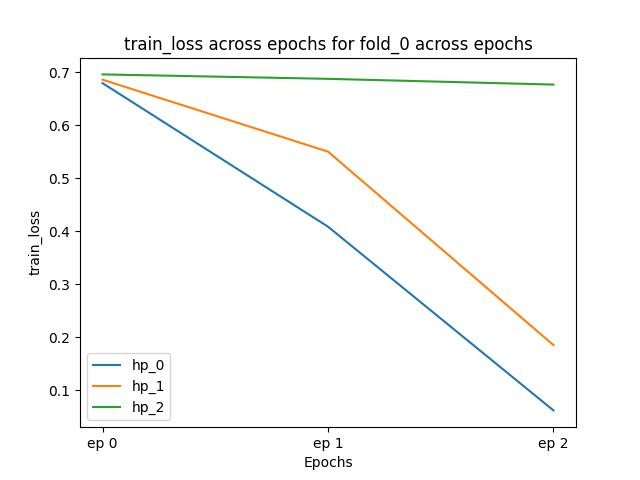
\includegraphics[scale = 0.75]{fold_0/train_loss}
\end{figure}
\subsection{test\_loss}
\begin{tabular}{lrrr}
\toprule
{} &   ep 0 &   ep 1 &   ep 2 \\
\midrule
hp\_0 &  0.642 &  0.462 &  0.505 \\
hp\_1 &  0.676 &  0.608 &  0.486 \\
hp\_2 &  0.691 &  0.687 &  0.681 \\
\bottomrule
\end{tabular}

\begin{figure}[H]
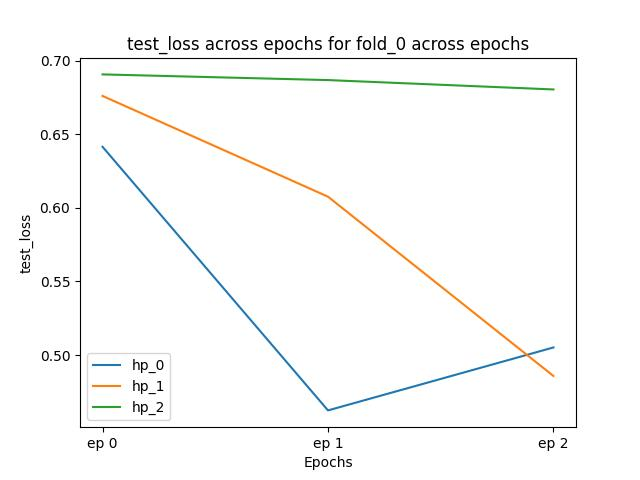
\includegraphics[scale = 0.75]{fold_0/test_loss}
\end{figure}
\subsection{accuracy\_score}
\begin{tabular}{lrrr}
\toprule
{} &   ep 0 &   ep 1 &   ep 2 \\
\midrule
hp\_0 &  0.667 &  0.803 &  0.812 \\
hp\_1 &  0.675 &  0.684 &  0.795 \\
hp\_2 &  0.521 &  0.692 &  0.701 \\
\bottomrule
\end{tabular}

\begin{figure}[H]
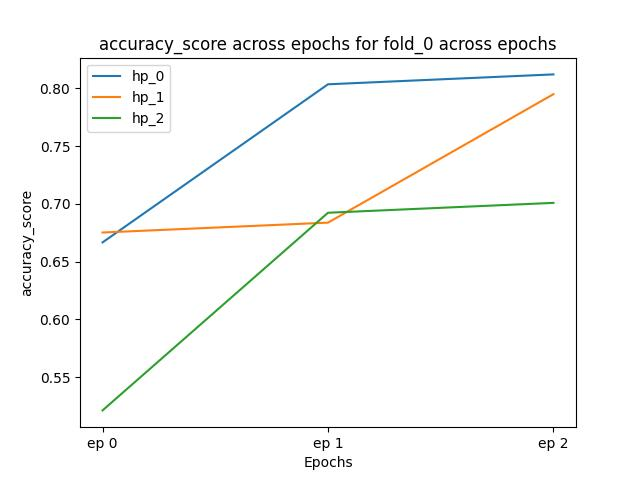
\includegraphics[scale = 0.75]{fold_0/accuracy_score}
\end{figure}
\subsection{f1\_score}
\begin{tabular}{lrrr}
\toprule
{} &   ep 0 &   ep 1 &   ep 2 \\
\midrule
hp\_0 &  0.738 &  0.827 &  0.804 \\
hp\_1 &  0.635 &  0.752 &  0.815 \\
hp\_2 &  0.674 &  0.700 &  0.624 \\
\bottomrule
\end{tabular}

\begin{figure}[H]
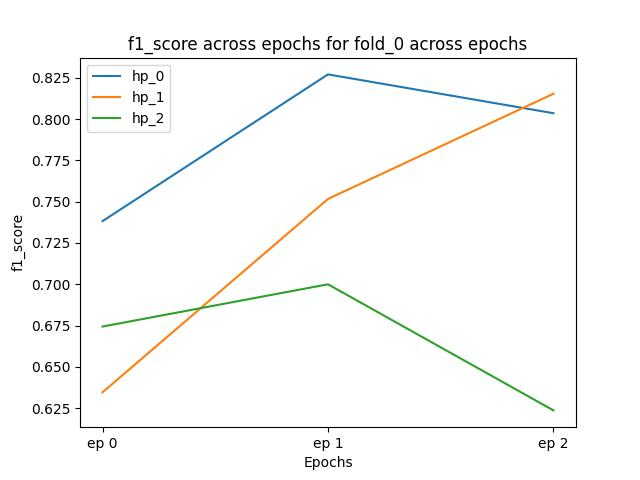
\includegraphics[scale = 0.75]{fold_0/f1_score}
\end{figure}
\subsection{precision\_score}
\begin{tabular}{lrrr}
\toprule
{} &   ep 0 &   ep 1 &   ep 2 \\
\midrule
hp\_0 &  0.604 &  0.733 &  0.833 \\
hp\_1 &  0.717 &  0.615 &  0.736 \\
hp\_2 &  0.509 &  0.677 &  0.829 \\
\bottomrule
\end{tabular}

\begin{figure}[H]
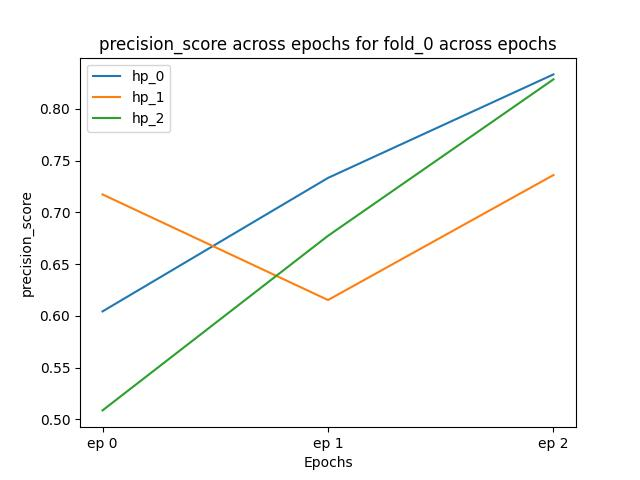
\includegraphics[scale = 0.75]{fold_0/precision_score}
\end{figure}
\subsection{matthews\_corrcoef}
\begin{tabular}{lrrr}
\toprule
{} &   ep 0 &   ep 1 &   ep 2 \\
\midrule
hp\_0 &  0.407 &  0.635 &  0.625 \\
hp\_1 &  0.357 &  0.448 &  0.608 \\
hp\_2 &  0.161 &  0.386 &  0.435 \\
\bottomrule
\end{tabular}

\begin{figure}[H]
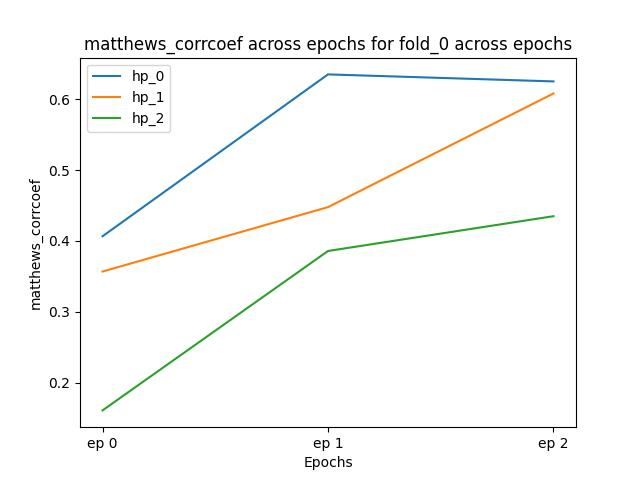
\includegraphics[scale = 0.75]{fold_0/matthews_corrcoef}
\end{figure}
\subsection{recall\_score}
\begin{tabular}{lrrr}
\toprule
{} &   ep 0 &   ep 1 &   ep 2 \\
\midrule
hp\_0 &  0.948 &  0.948 &  0.776 \\
hp\_1 &  0.569 &  0.966 &  0.914 \\
hp\_2 &  1.000 &  0.724 &  0.500 \\
\bottomrule
\end{tabular}

\begin{figure}[H]
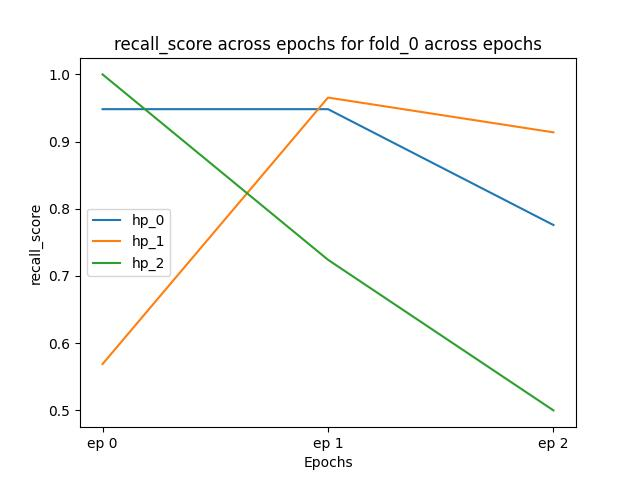
\includegraphics[scale = 0.75]{fold_0/recall_score}
\end{figure}
\section{fold\_1}
\subsection{train\_loss}
\begin{tabular}{lrrr}
\toprule
{} &   ep 0 &   ep 1 &   ep 2 \\
\midrule
hp\_0 &  0.680 &  0.465 &  0.107 \\
hp\_1 &  0.685 &  0.523 &  0.142 \\
hp\_2 &  0.690 &  0.683 &  0.672 \\
\bottomrule
\end{tabular}

\begin{figure}[H]
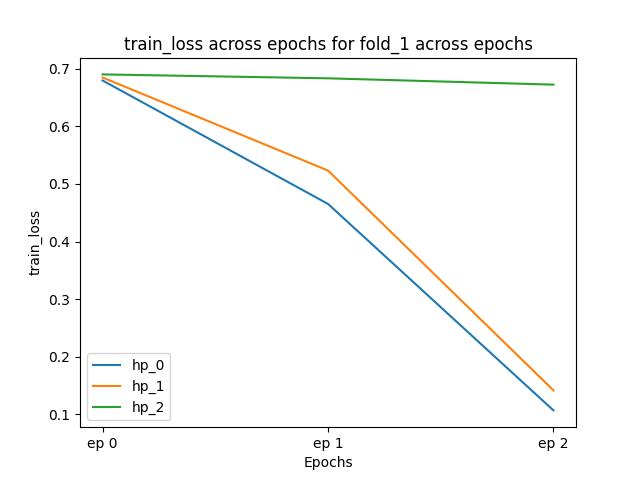
\includegraphics[scale = 0.75]{fold_1/train_loss}
\end{figure}
\subsection{test\_loss}
\begin{tabular}{lrrr}
\toprule
{} &   ep 0 &   ep 1 &   ep 2 \\
\midrule
hp\_0 &  0.618 &  0.394 &  0.422 \\
hp\_1 &  0.673 &  0.411 &  0.403 \\
hp\_2 &  0.693 &  0.690 &  0.683 \\
\bottomrule
\end{tabular}

\begin{figure}[H]
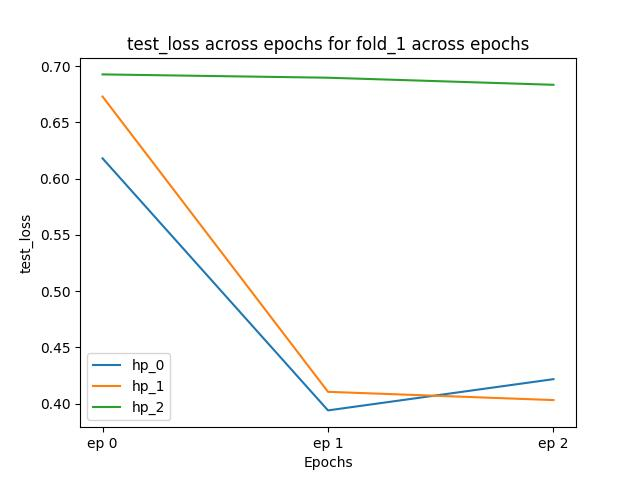
\includegraphics[scale = 0.75]{fold_1/test_loss}
\end{figure}
\subsection{accuracy\_score}
\begin{tabular}{lrrr}
\toprule
{} &   ep 0 &   ep 1 &   ep 2 \\
\midrule
hp\_0 &  0.741 &  0.828 &  0.828 \\
hp\_1 &  0.672 &  0.784 &  0.810 \\
hp\_2 &  0.483 &  0.483 &  0.483 \\
\bottomrule
\end{tabular}

\begin{figure}[H]
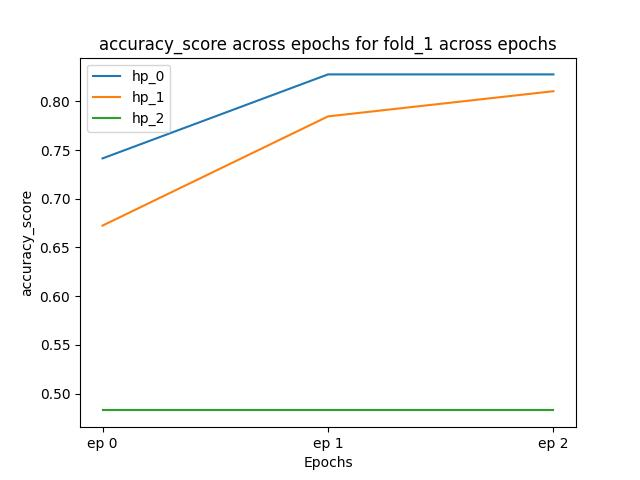
\includegraphics[scale = 0.75]{fold_1/accuracy_score}
\end{figure}
\subsection{f1\_score}
\begin{tabular}{lrrr}
\toprule
{} &   ep 0 &   ep 1 &   ep 2 \\
\midrule
hp\_0 &  0.732 &  0.828 &  0.839 \\
hp\_1 &  0.568 &  0.779 &  0.817 \\
hp\_2 &  0.000 &  0.000 &  0.000 \\
\bottomrule
\end{tabular}

\begin{figure}[H]
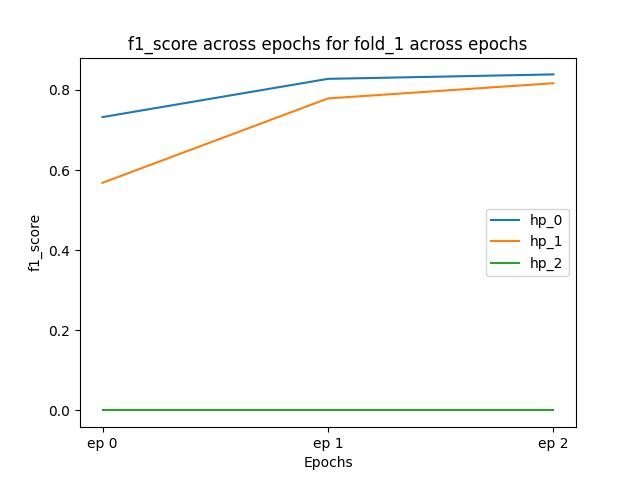
\includegraphics[scale = 0.75]{fold_1/f1_score}
\end{figure}
\subsection{precision\_score}
\begin{tabular}{lrrr}
\toprule
{} &   ep 0 &   ep 1 &   ep 2 \\
\midrule
hp\_0 &  0.788 &  0.857 &  0.812 \\
hp\_1 &  0.893 &  0.830 &  0.817 \\
hp\_2 &  0.000 &  0.000 &  0.000 \\
\bottomrule
\end{tabular}

\begin{figure}[H]
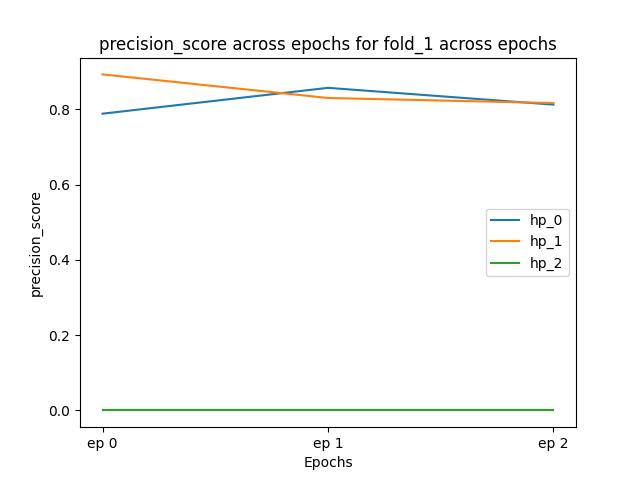
\includegraphics[scale = 0.75]{fold_1/precision_score}
\end{figure}
\subsection{matthews\_corrcoef}
\begin{tabular}{lrrr}
\toprule
{} &   ep 0 &   ep 1 &   ep 2 \\
\midrule
hp\_0 &  0.489 &  0.657 &  0.656 \\
hp\_1 &  0.424 &  0.574 &  0.620 \\
hp\_2 &  0.000 &  0.000 &  0.000 \\
\bottomrule
\end{tabular}

\begin{figure}[H]
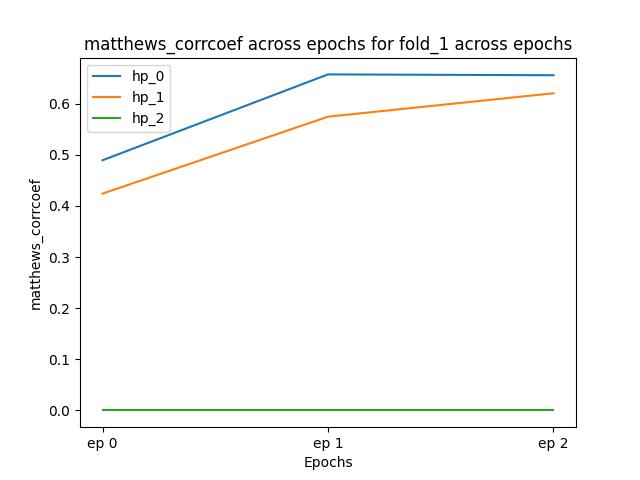
\includegraphics[scale = 0.75]{fold_1/matthews_corrcoef}
\end{figure}
\subsection{recall\_score}
\begin{tabular}{lrrr}
\toprule
{} &   ep 0 &   ep 1 &   ep 2 \\
\midrule
hp\_0 &  0.683 &  0.800 &  0.867 \\
hp\_1 &  0.417 &  0.733 &  0.817 \\
hp\_2 &  0.000 &  0.000 &  0.000 \\
\bottomrule
\end{tabular}

\begin{figure}[H]
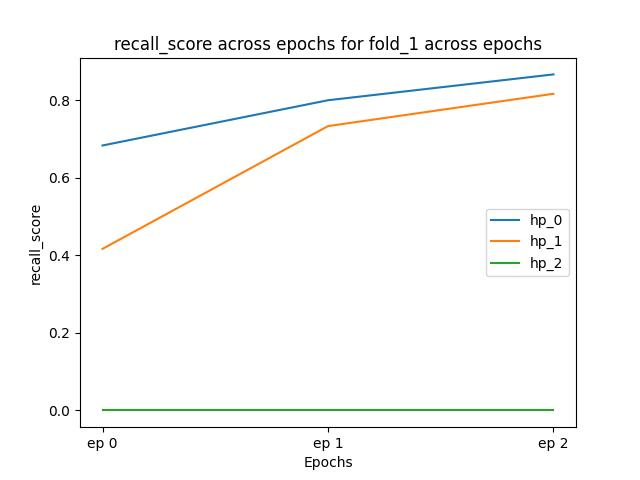
\includegraphics[scale = 0.75]{fold_1/recall_score}
\end{figure}
\section{fold\_2}
\subsection{train\_loss}
\begin{tabular}{lrrr}
\toprule
{} &   ep 0 &   ep 1 &   ep 2 \\
\midrule
hp\_0 &  0.695 &  0.432 &  0.054 \\
hp\_1 &  0.693 &  0.586 &  0.170 \\
hp\_2 &  0.694 &  0.689 &  0.680 \\
\bottomrule
\end{tabular}

\begin{figure}[H]
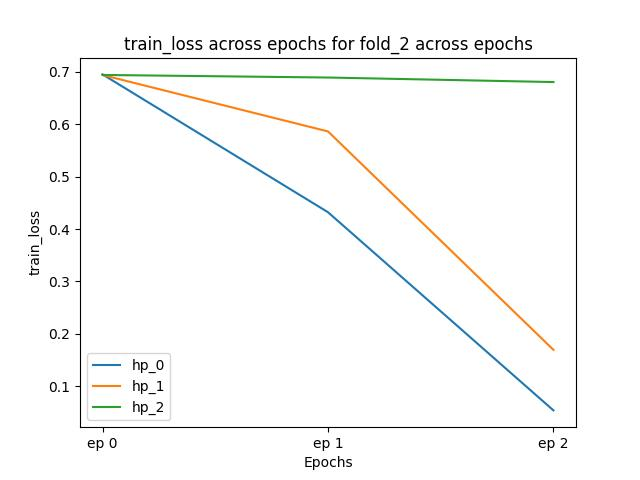
\includegraphics[scale = 0.75]{fold_2/train_loss}
\end{figure}
\subsection{test\_loss}
\begin{tabular}{lrrr}
\toprule
{} &   ep 0 &   ep 1 &   ep 2 \\
\midrule
hp\_0 &  0.661 &  0.382 &  0.242 \\
hp\_1 &  0.676 &  0.464 &  0.479 \\
hp\_2 &  0.693 &  0.689 &  0.682 \\
\bottomrule
\end{tabular}

\begin{figure}[H]
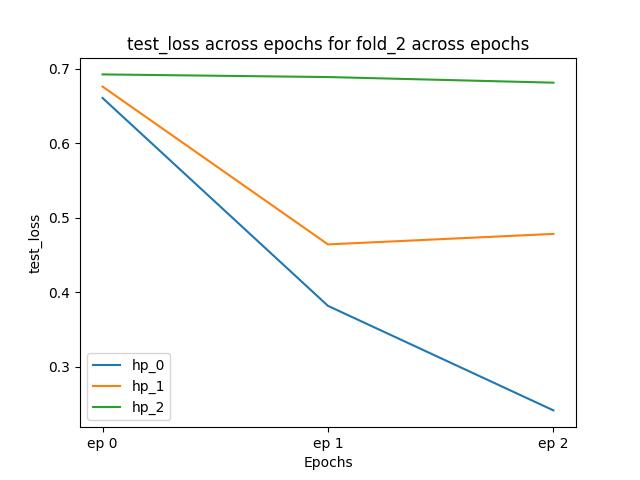
\includegraphics[scale = 0.75]{fold_2/test_loss}
\end{figure}
\subsection{accuracy\_score}
\begin{tabular}{lrrr}
\toprule
{} &   ep 0 &   ep 1 &   ep 2 \\
\midrule
hp\_0 &  0.862 &  0.836 &  0.914 \\
hp\_1 &  0.733 &  0.845 &  0.802 \\
hp\_2 &  0.517 &  0.603 &  0.690 \\
\bottomrule
\end{tabular}

\begin{figure}[H]
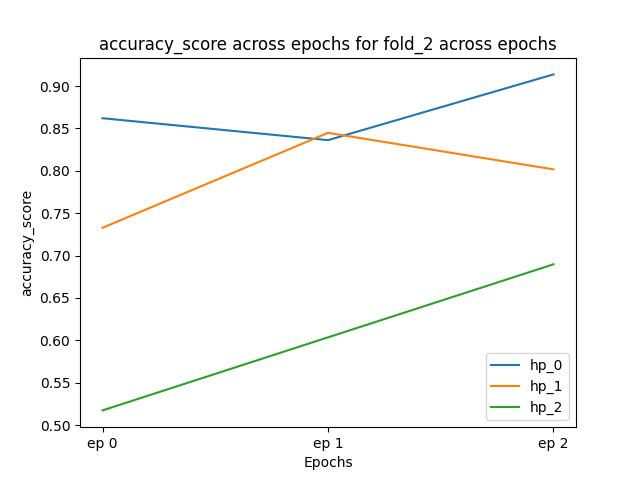
\includegraphics[scale = 0.75]{fold_2/accuracy_score}
\end{figure}
\subsection{f1\_score}
\begin{tabular}{lrrr}
\toprule
{} &   ep 0 &   ep 1 &   ep 2 \\
\midrule
hp\_0 &  0.822 &  0.832 &  0.894 \\
hp\_1 &  0.744 &  0.836 &  0.800 \\
hp\_2 &  0.569 &  0.657 &  0.710 \\
\bottomrule
\end{tabular}

\begin{figure}[H]
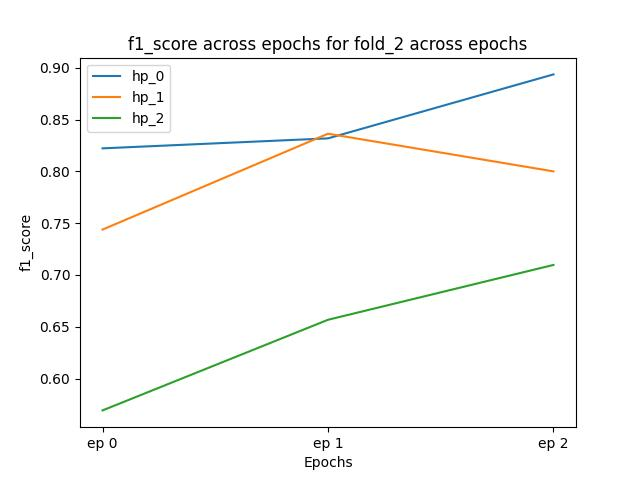
\includegraphics[scale = 0.75]{fold_2/f1_score}
\end{figure}
\subsection{precision\_score}
\begin{tabular}{lrrr}
\toprule
{} &   ep 0 &   ep 1 &   ep 2 \\
\midrule
hp\_0 &  0.881 &  0.723 &  0.913 \\
hp\_1 &  0.616 &  0.742 &  0.687 \\
hp\_2 &  0.451 &  0.512 &  0.579 \\
\bottomrule
\end{tabular}

\begin{figure}[H]
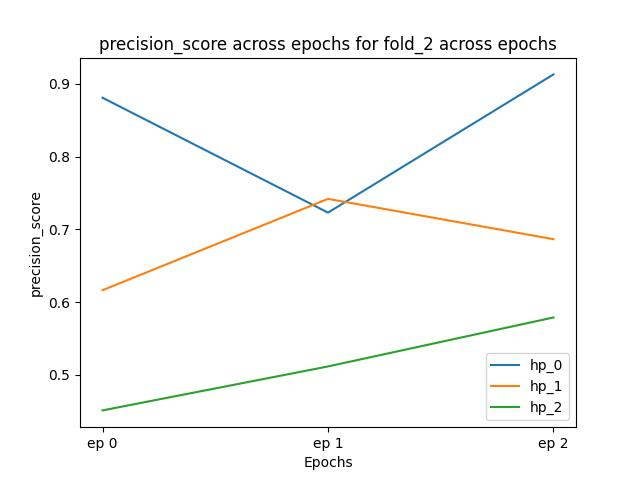
\includegraphics[scale = 0.75]{fold_2/precision_score}
\end{figure}
\subsection{matthews\_corrcoef}
\begin{tabular}{lrrr}
\toprule
{} &   ep 0 &   ep 1 &   ep 2 \\
\midrule
hp\_0 &  0.715 &  0.709 &  0.822 \\
hp\_1 &  0.536 &  0.714 &  0.648 \\
hp\_2 &  0.118 &  0.336 &  0.462 \\
\bottomrule
\end{tabular}

\begin{figure}[H]
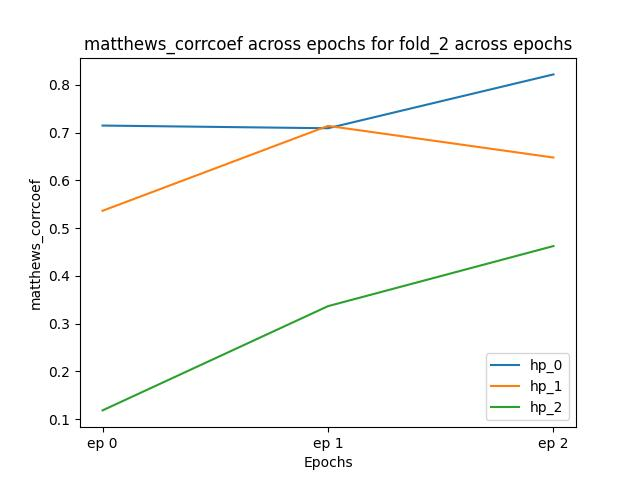
\includegraphics[scale = 0.75]{fold_2/matthews_corrcoef}
\end{figure}
\subsection{recall\_score}
\begin{tabular}{lrrr}
\toprule
{} &   ep 0 &   ep 1 &   ep 2 \\
\midrule
hp\_0 &  0.771 &  0.979 &  0.875 \\
hp\_1 &  0.938 &  0.958 &  0.958 \\
hp\_2 &  0.771 &  0.917 &  0.917 \\
\bottomrule
\end{tabular}

\begin{figure}[H]
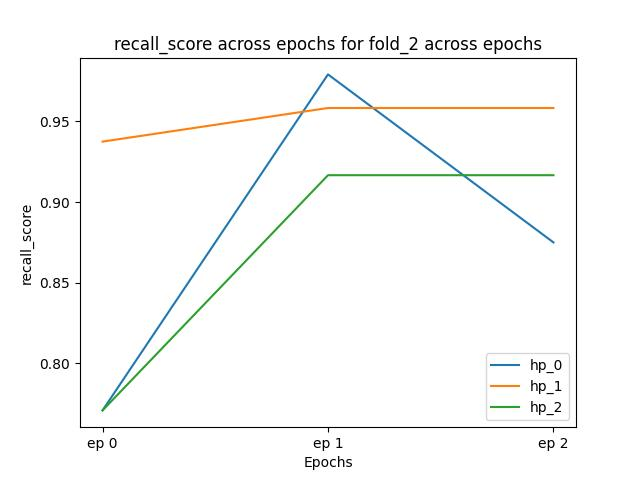
\includegraphics[scale = 0.75]{fold_2/recall_score}
\end{figure}
\end{document}
